% Created 2018-10-01 Mon 14:33
% Intended LaTeX compiler: pdflatex
\documentclass[10pt,t]{beamer}
\usepackage[utf8]{inputenc}
\usepackage[T1]{fontenc}
\usepackage{graphicx}
\usepackage{grffile}
\usepackage{longtable}
\usepackage{wrapfig}
\usepackage{rotating}
\usepackage[normalem]{ulem}
\usepackage{amsmath}
\usepackage{textcomp}
\usepackage{amssymb}
\usepackage{capt-of}
\usepackage{hyperref}
\usetheme{default}
\author{L. Larrabee Strow}
\date{\today}
\title{\large A Climate Hyperspectral InfraRed Product (CHIRP)}
\date{\textit{\footnotesize June 20, 2018}}
\input beamer_setup
\usetheme{metropolis}
\metroset{titleformat title=allcaps}
\renewcommand{\UrlFont}{\small\tt}
\renewcommand*{\UrlFont}{\footnotesize}
\tolerance=1000
\RequirePackage{fancyvrb}
\DefineVerbatimEnvironment{verbatim}{Verbatim}{fontsize=\footnotesize}
\subtitle{\footnotesize AKA:  A Long-Term Homogeneous Hyperspectral Radiance Time Series: AIRS2CrIS}
\author{L.~Larrabee~Strow and Howard~Motteler (UMBC)}
\definecolor{mAlert}{rgb}{0.4824 0.0667 0.0745}
\hypersetup{
 pdfauthor={L. Larrabee Strow},
 pdftitle={\large A Climate Hyperspectral InfraRed Product (CHIRP)},
 pdfkeywords={},
 pdfsubject={},
 pdfcreator={Emacs 25.3.1 (Org mode 9.1.12)}, 
 pdflang={English}}
\begin{document}

\maketitle
\addtobeamertemplate{block begin}{
  \setlength{\parsep}{0pt}
  \setlength{\topsep}{3pt plus 2pt minus 2.5pt}
  \setlength{\itemsep}{0pt plus 0pt minus 2pt}
  \setlength{\partopsep}{2pt}
}

\begin{frame}[shrink=20,label={sec:orga86e1c0}]{Introduction}
\vspace{-0.1in}

\begin{itemize}
\item We have a mult-instrument hyperspectral radiance record (AIRS, CrIS(2), IASI(2)
\item NASA has asked for continuity products, with an emphasis on climate
\item For climate, the radiances are a "product" used by the scientific community
\end{itemize}
\begin{block}{Instrument Characteristics (AIRS vs CrIS vs IASI)}
\begin{itemize}
\item Different Spectral Response Functions (SRF)
\item Different channel center frequencies (\(\nu_i\))
\item Different, but similar absolute calibration accuracy (\textasciitilde{}0.1-0.3K)
\item BUT: \emph{Their radiometric stability is at least \textasciitilde{}100 X \alert{BETTER} then absolute calibration accuracy!}
\end{itemize}
\end{block}
\begin{block}{Possible Continuity Requirements (that provide same observation sensitivities)}
\begin{itemize}
\item Same SRFs
\item Same \(\nu_i\)
\item Same Radiative transfer model (RTA)
\item Same noise?
\item Same retrieval algorithm
\end{itemize}

\large Proposed Solution: \textcolor{maroon}{CHIRP}
\end{block}
\end{frame}

\begin{frame}[label={sec:org5258a0c}]{CHIRP + Radiance Based L3 Retrieval Data Flow}
\begin{center}
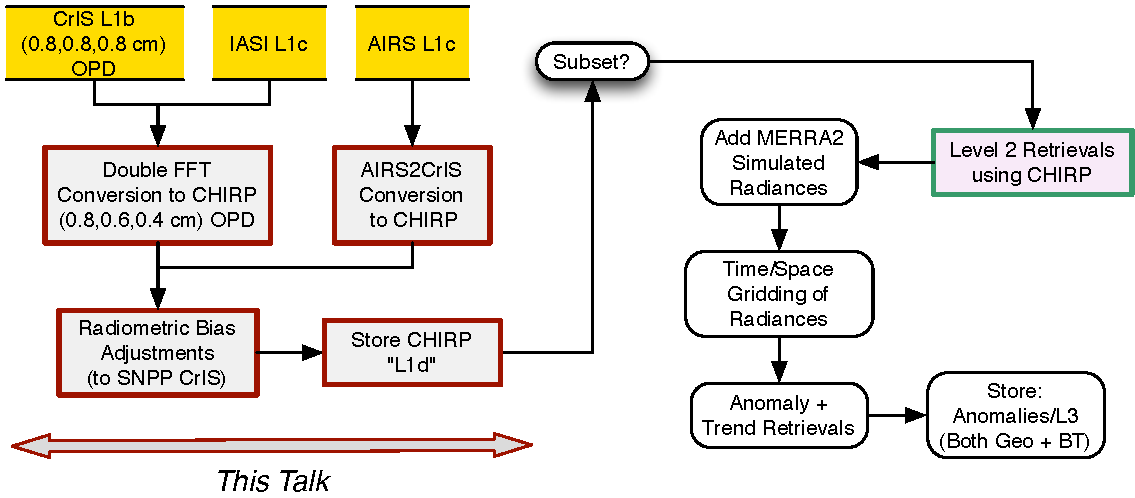
\includegraphics[width=1.0\linewidth]{./Figs/Pdf/airs2cris_stm_talk1_landscape.pdf}
\end{center}

\begin{itemize}
\item \emph{OPD:} Close to 0.8 / 0.6 /0.4 cm
\item \emph{With Spectral Spacing:} 0.0625 / 0.0833 / 0.1250 \wn
\end{itemize}

Requirement: High-quality conversion of AIRS to CHIRP ILS

CHIRP = (1) AIRS2CrIS (2) CrIS modified SRF, (3) IASI modified SRF
\end{frame}

\begin{frame}[label={sec:org9f1e524}]{CHIRP only Data Flow: Useful for Level 2 Retrievals?}
\vspace{-0.1in}

\begin{center}
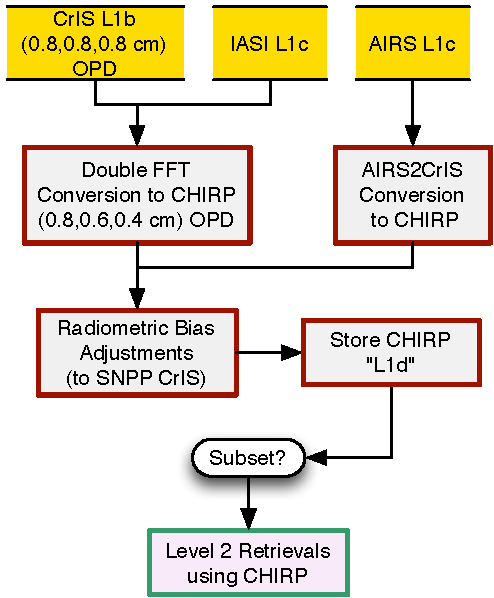
\includegraphics[width=0.6\linewidth]{./Figs/Pdf/airs2cris_stm_talk1_small.pdf}
\end{center}

\vspace{-0.1in}
\end{frame}

\begin{frame}[label={sec:orgae15ba2}]{AIRS2CrIS Algorithm}
\vspace{-0.15in}
\begin{small}
\begin{itemize}
\item Simple deconvolution to 0.1 \wn grid
\item \(S_a r = r_A\), \(r_o = S_a^{-1} r_A\) using Moore-Penrose pseudoinverse
\item \(r_{A2C} = S_c \circledast r_o\)
\item Small additional terms using linear regression (mostly bias)
\item Errors below assume AIRS ILS functions are perfect
\end{itemize}
\end{small}
\vspace{-0.25in}
\begin{columns}
\begin{column}{0.55\columnwidth}
\begin{block}{\footnotesize AIRS2CrIS Mean Error (std. similar)}
\vspace{-0.1in}
\begin{center}
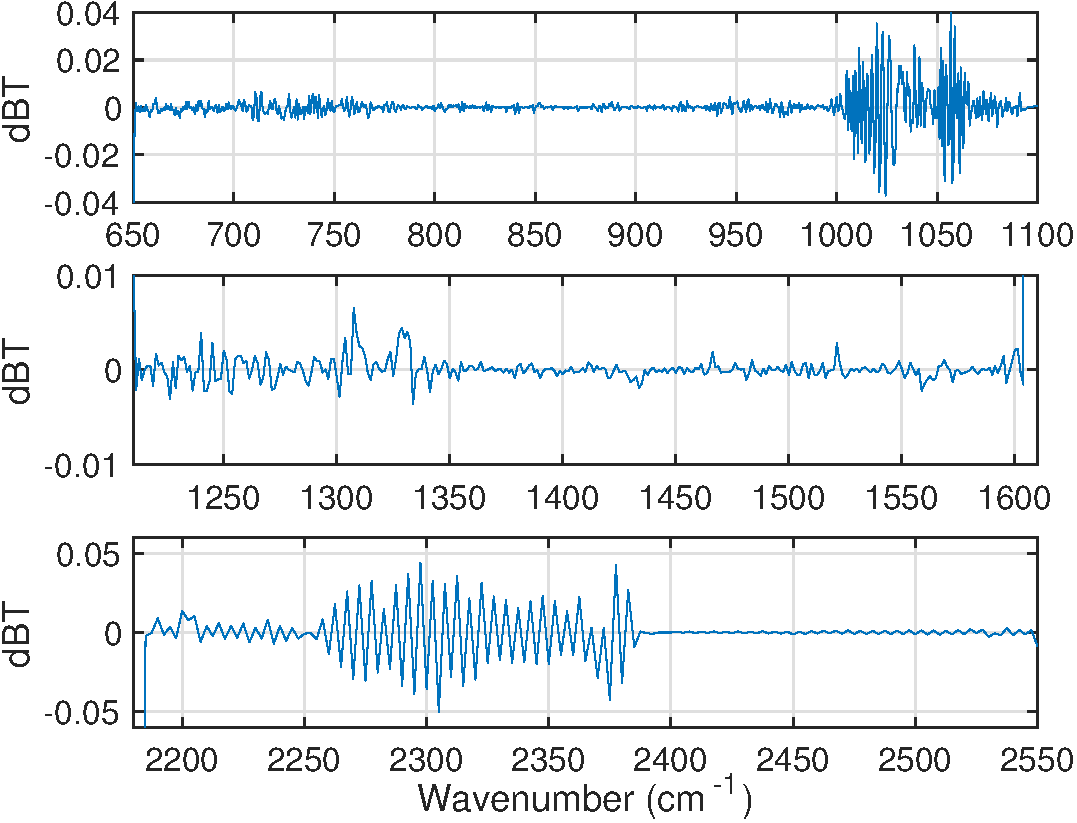
\includegraphics[width=0.95\linewidth]{./Figs/Pdf/ap_decon_corr.pdf}
\end{center}
\end{block}
\end{column}

\begin{column}{0.55\columnwidth}
\begin{block}{\footnotesize AIRS2CrIS Noise}
\vspace{-0.1in}
\begin{center}
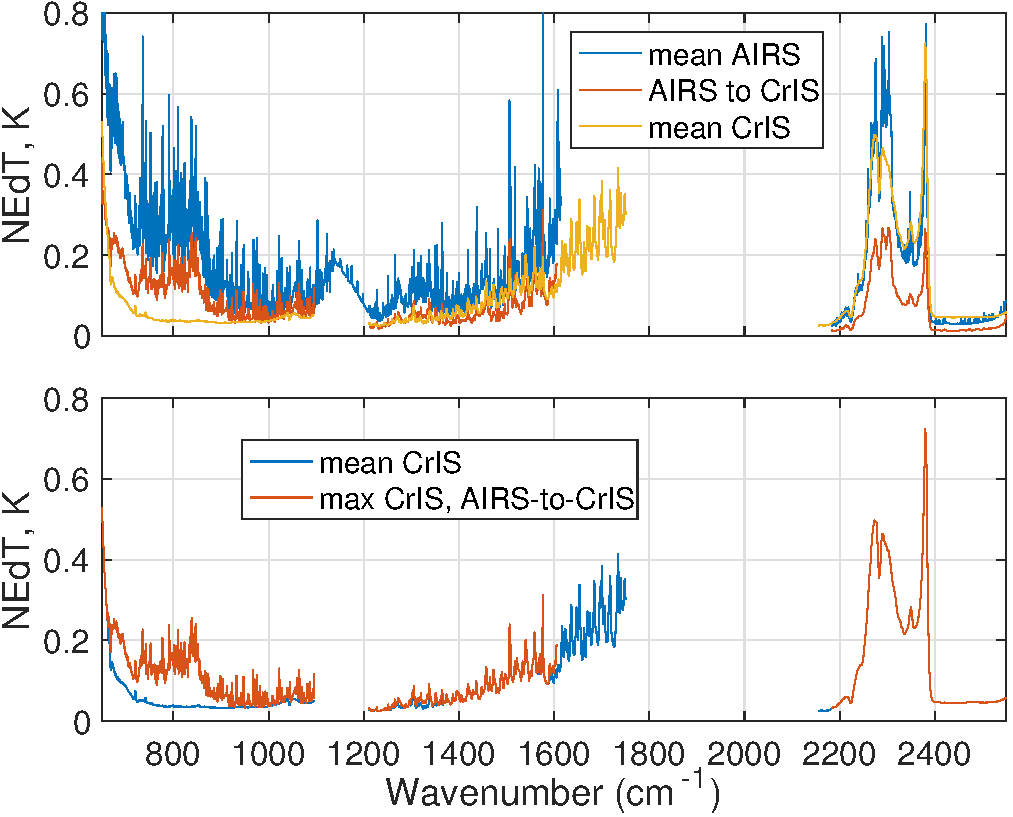
\includegraphics[width=0.95\linewidth]{./Figs/Pdf/a2cris_nedt.pdf}
\end{center}
\end{block}
\end{column}
\end{columns}

\vspace{-0.1in}
\small Shortwave sounding region max noise dominated by CrIS
\end{frame}

\begin{frame}[label={sec:org8da6082}]{Spectral Differences Among AIRS, CrIS, IASI}
\vspace{-0.2in}
\begin{columns}
\begin{column}{0.55\columnwidth}
\begin{block}{AIRS/CrIS/IASI Spectra}
\begin{center}
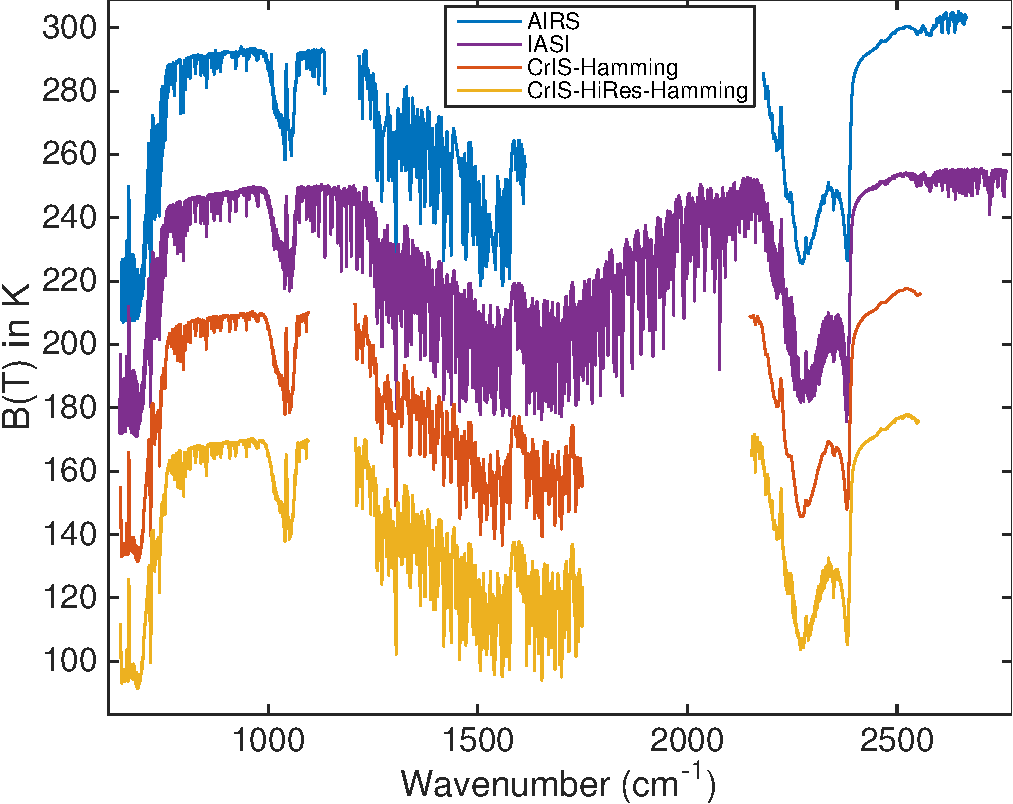
\includegraphics[width=\linewidth]{./Figs/Pdf/hyperall_hamming.pdf}
\end{center}
\end{block}
\end{column}


\begin{column}{0.55\columnwidth}
\begin{block}{CHIRP Spectrum (from AIRS)}
\begin{center}
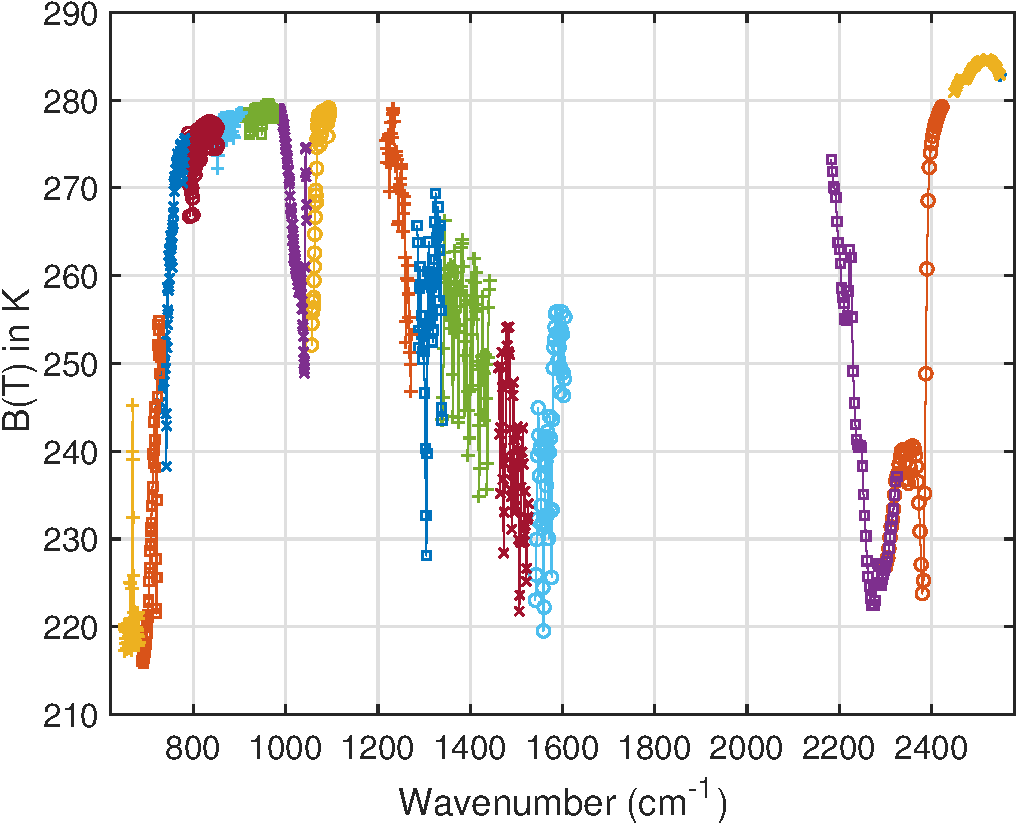
\includegraphics[width=\linewidth]{./Figs/Pdf/a2c_full.pdf}
\end{center}
\end{block}
\end{column}
\end{columns}

AIRS modules shown in different colors in CHIRP spectrum. This is CrIS-NSR, final CHIRP will be between CrIS NSR and FSR (MW/SW).
\end{frame}

\begin{frame}[label={sec:orgd9668e0}]{Bad CHIRP Channels are Flagged}
\vspace{-0.35in}
\begin{columns}
\begin{column}{0.55\columnwidth}
\begin{block}{\footnotesize Simulated Channels}
\vspace{-0.05in}
\vspace{-0.05in}
\begin{center}
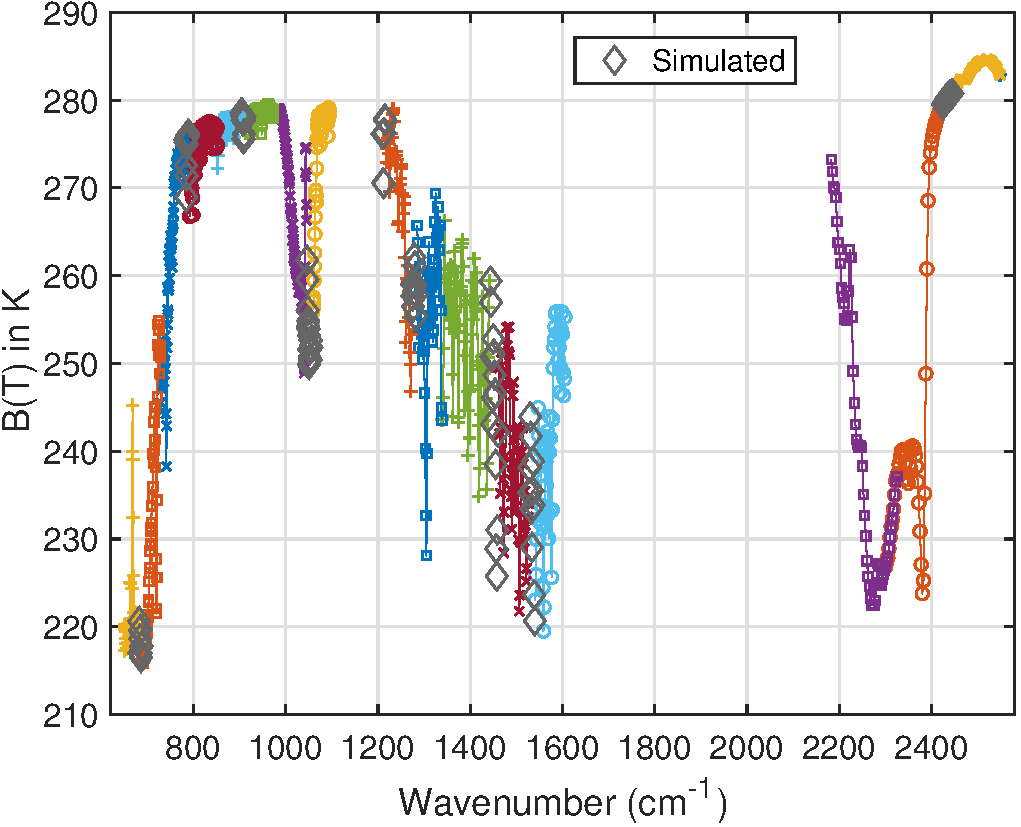
\includegraphics[width=0.77\linewidth]{./Figs/Pdf/a2c_full_show_sim.pdf}
\end{center}
\end{block}
\end{column}

\begin{column}{0.55\columnwidth}
\begin{block}{\footnotesize Dead Channels}
\vspace{-0.05in}
\vspace{-0.05in}
\begin{center}
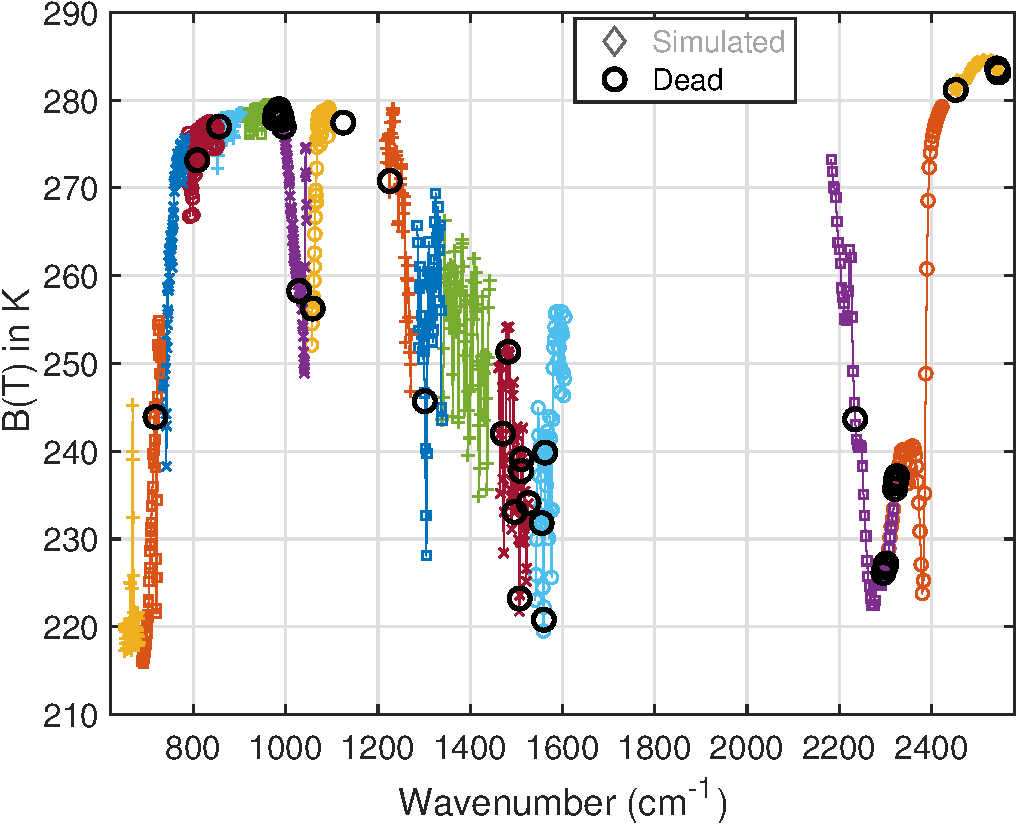
\includegraphics[width=0.77\linewidth]{./Figs/Pdf/a2c_full_show_dead.pdf}
\end{center}
\end{block}
\end{column}
\end{columns}

\vspace{-0.25in}

\begin{columns}
\begin{column}{0.55\columnwidth}
\begin{block}{\footnotesize Noisy Channels}
\vspace{-0.05in}
\vspace{-0.05in}
\begin{center}
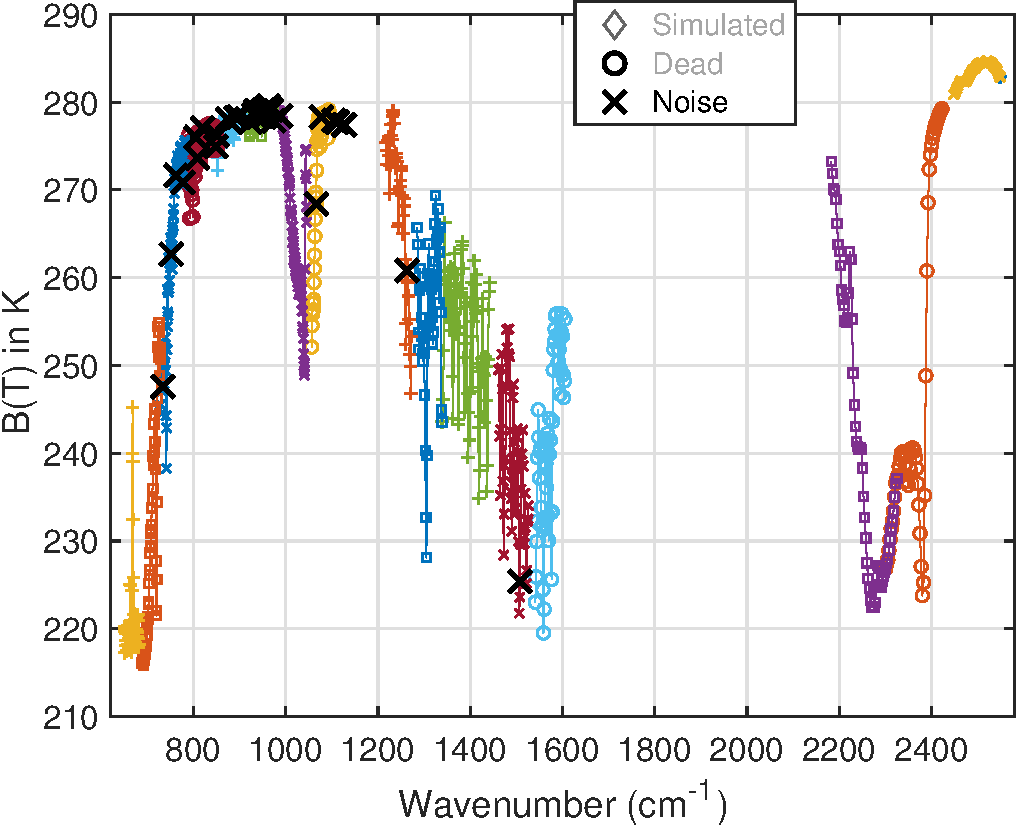
\includegraphics[width=0.77\linewidth]{./Figs/Pdf/a2c_full_show_noise.pdf}
\end{center}
\end{block}
\end{column}

\begin{column}{0.55\columnwidth}
\begin{block}{\footnotesize Midwave Zoom: Dead and Noisy Chanels}
\vspace{-0.05in}
\vspace{-0.05in}
\begin{center}
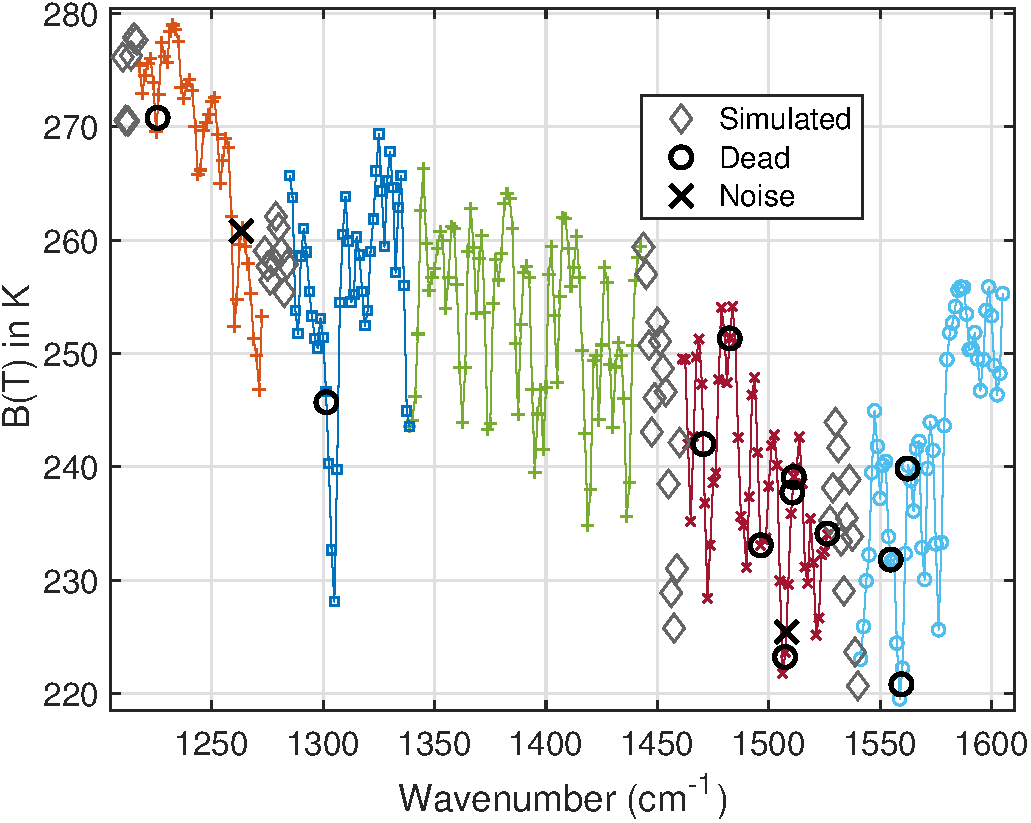
\includegraphics[width=0.77\linewidth]{./Figs/Pdf/a2c_full_show_dead_noise_water.pdf}
\end{center}
\end{block}
\end{column}
\end{columns}
\end{frame}

\begin{frame}[label={sec:orgabf5fb7}]{Validation: PDF's of Single Channels}
\begin{itemize}
\item How closely will AIRS2CrIS (CHIRP) compare to CrIS for single scenes?
\item We collected a large random statistical set of AIRS and SNPP-CrIS observations for the 675.6 \wn channels (closest matches)
\item Examine the PDFs (histograms) of (a) AIRS native SRF (b) AIRS2CrIS, with (c) CrIS.
\end{itemize}
\end{frame}

\begin{frame}[label={sec:org3f462d9}]{PDF's for a Single CHIRP Channel Compared to CrIS}
\vspace{-0.35in}
\begin{columns}
\begin{column}{0.55\columnwidth}
\begin{block}{\footnotesize AIRS only, Noise added}
\vspace{-0.05in}
\vspace{-0.05in}
\begin{center}
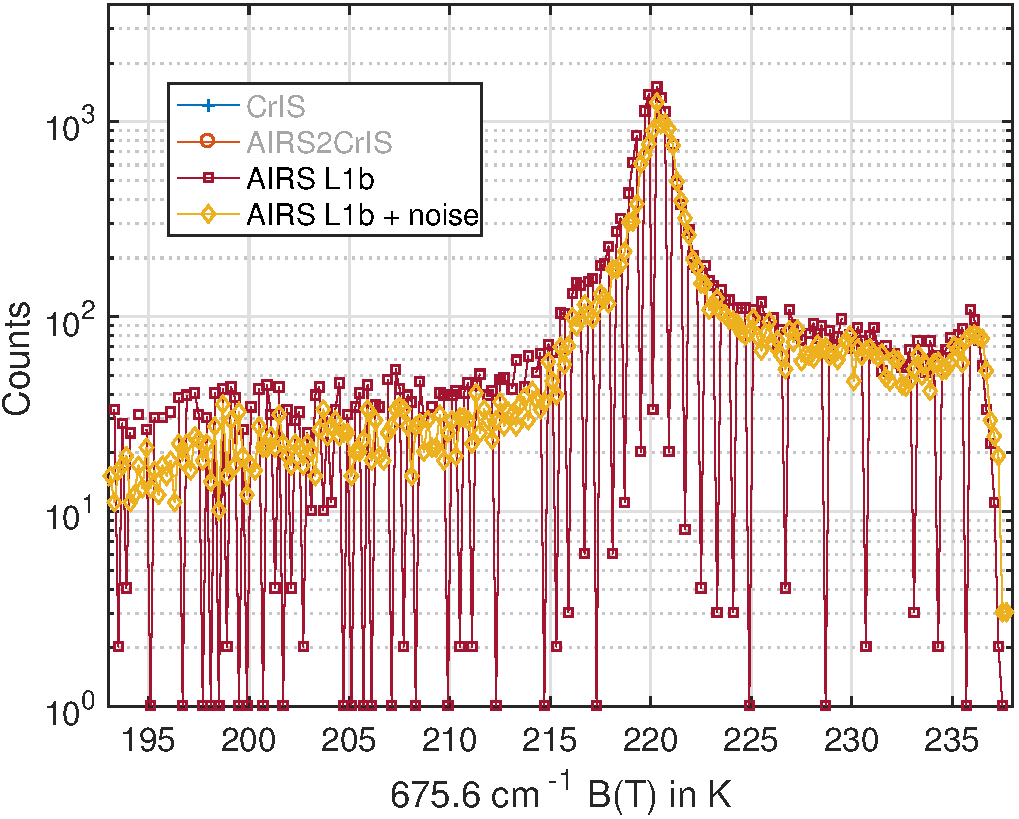
\includegraphics[width=0.77\linewidth]{./Figs/Pdf/jun4_2015_airs_675wn_global_counts_w_airsnoise.pdf}
\end{center}
\end{block}
\end{column}

\begin{column}{0.55\columnwidth}
\begin{block}{\footnotesize PDF for closest CrIS Channel}
\vspace{-0.05in}
\vspace{-0.05in}
\begin{center}
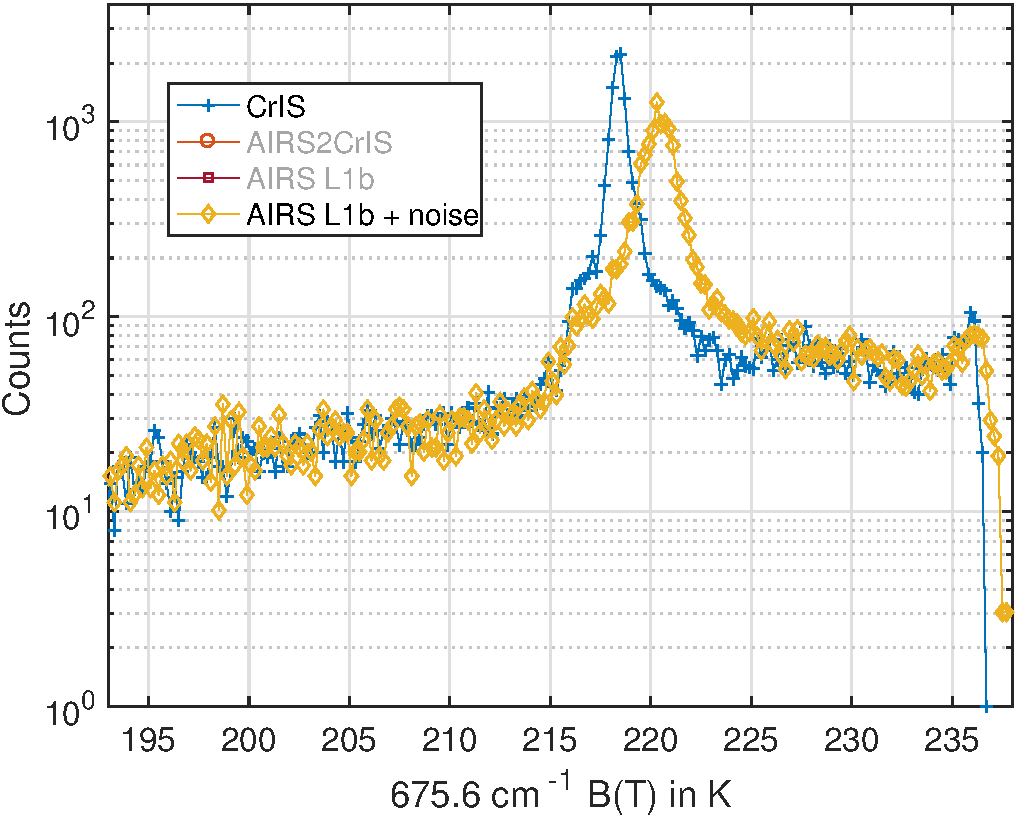
\includegraphics[width=0.77\linewidth]{./Figs/Pdf/jun4_2015_airs_675wn_global_counts_w_airsnoise_and_cris.pdf}
\end{center}
\end{block}
\end{column}
\end{columns}

\vspace{-0.25in}

\begin{columns}
\begin{column}{0.55\columnwidth}
\begin{block}{\footnotesize Convert AIRS to CrIS SRF}
\vspace{-0.05in}
\vspace{-0.05in}
\begin{center}
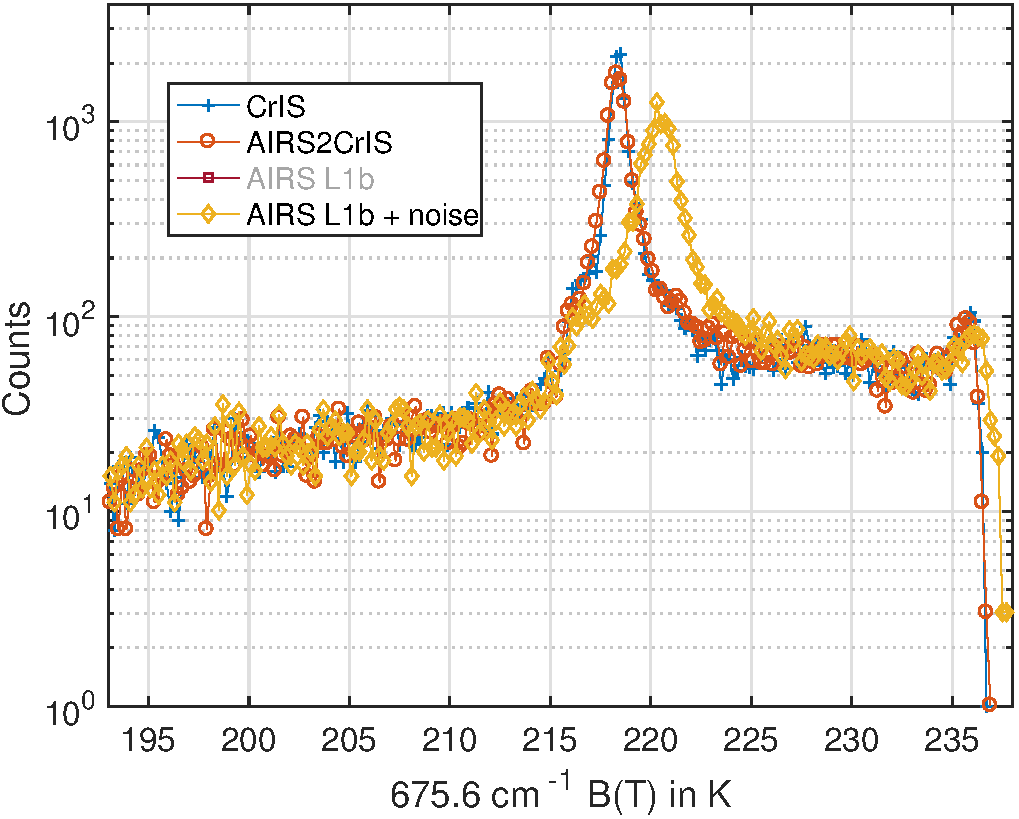
\includegraphics[width=0.77\linewidth]{./Figs/Pdf/jun4_2015_airs_675wn_global_counts_w_airsnoise_and_cris_a2c.pdf}
\end{center}
\end{block}
\end{column}

\begin{column}{0.55\columnwidth}
\begin{block}{\footnotesize CrIS versus CHIRP}
\vspace{-0.05in}
\vspace{-0.05in}
\begin{center}
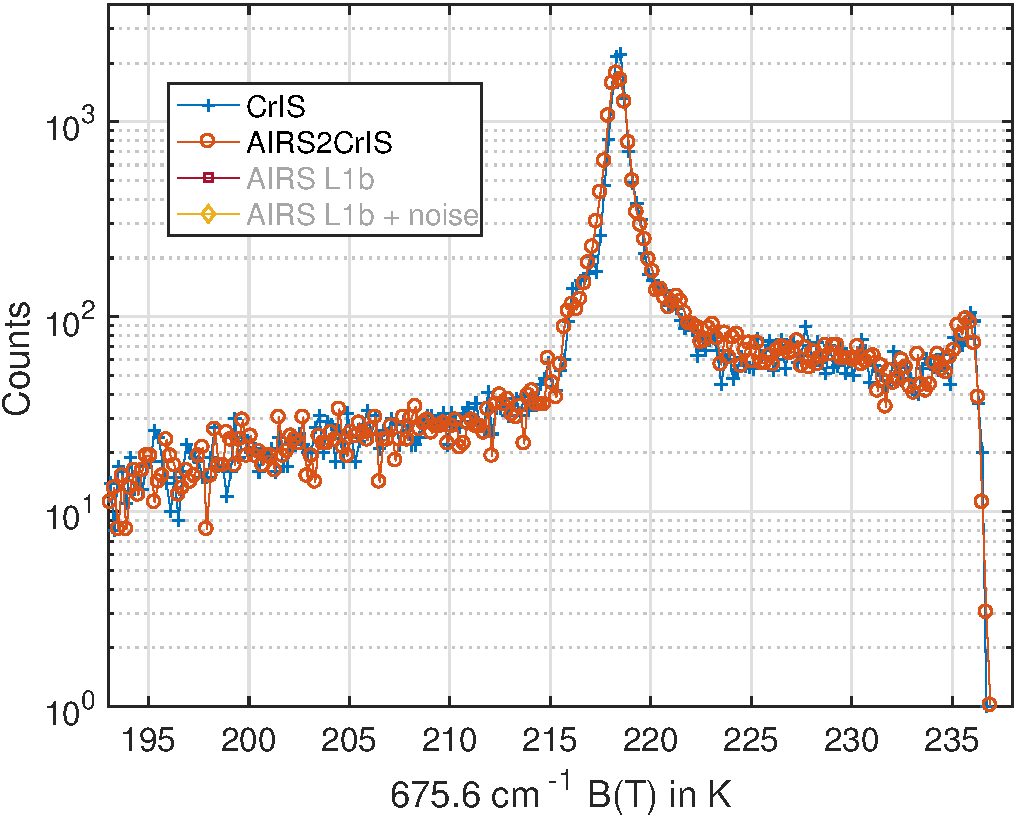
\includegraphics[width=0.77\linewidth]{./Figs/Pdf/jun4_2015_airs_675wn_global_counts_w_airsnoise_and_cris_a2c_no_airs.pdf}
\end{center}

:Beamer\_opt: shrink=20
\end{block}
\end{column}
\end{columns}
\end{frame}
\begin{frame}[label={sec:orgf9048bc}]{Validation: SNOs between CrIS and AIRS/CHIRP}
\begin{itemize}
\item SNOs are Simultaneous Nadir Overlaps
\item We generate them for combinations of AIRS, CrIS, and IASI
\item And convert AIRS to AIRS2CrIS (CHIRP)
\item Allows \emph{channel-by-channel} inter-comparisons (instrument offsets)
\item We also use AIRS2CrIS as a transfer standard to intercompare SNPP-CrIS to NOAA20-CrIS since SNPP and NOAA20 do not have nadir overlaps
\item See Chris Hepplewhite's talk on Friday for more details
\end{itemize}
\end{frame}

\begin{frame}[label={sec:orgdf10d64}]{SNPP versus AIRS: SNOs and Large Random Samplings}
\vspace{-0.3in}

\begin{columns}
\begin{column}{0.55\columnwidth}
\begin{block}{\footnotesize 2016 SNOs}
\vspace{-0.1in}
\begin{center}
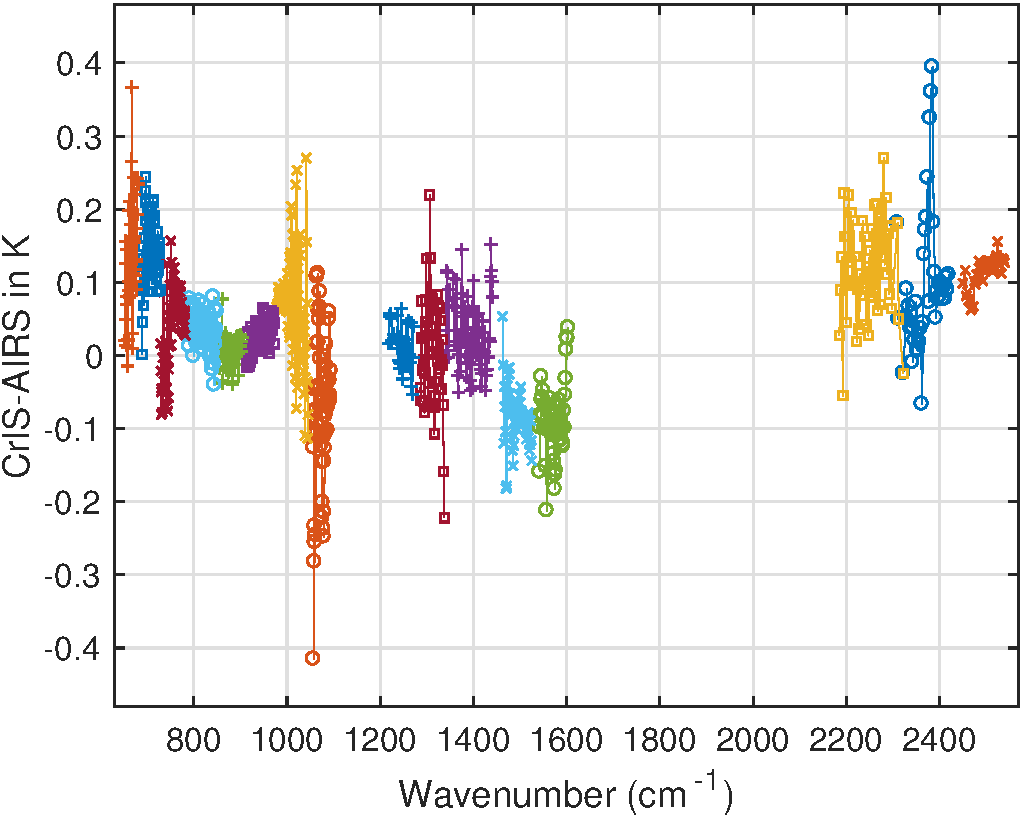
\includegraphics[width=\linewidth]{./Figs/Pdf/snpp_vs_airs_sno.pdf}
\end{center}
\end{block}
\end{column}

\begin{column}{0.55\columnwidth}
\begin{block}{\footnotesize 2016 Random Comparisons}
\vspace{-0.1in}
\begin{center}
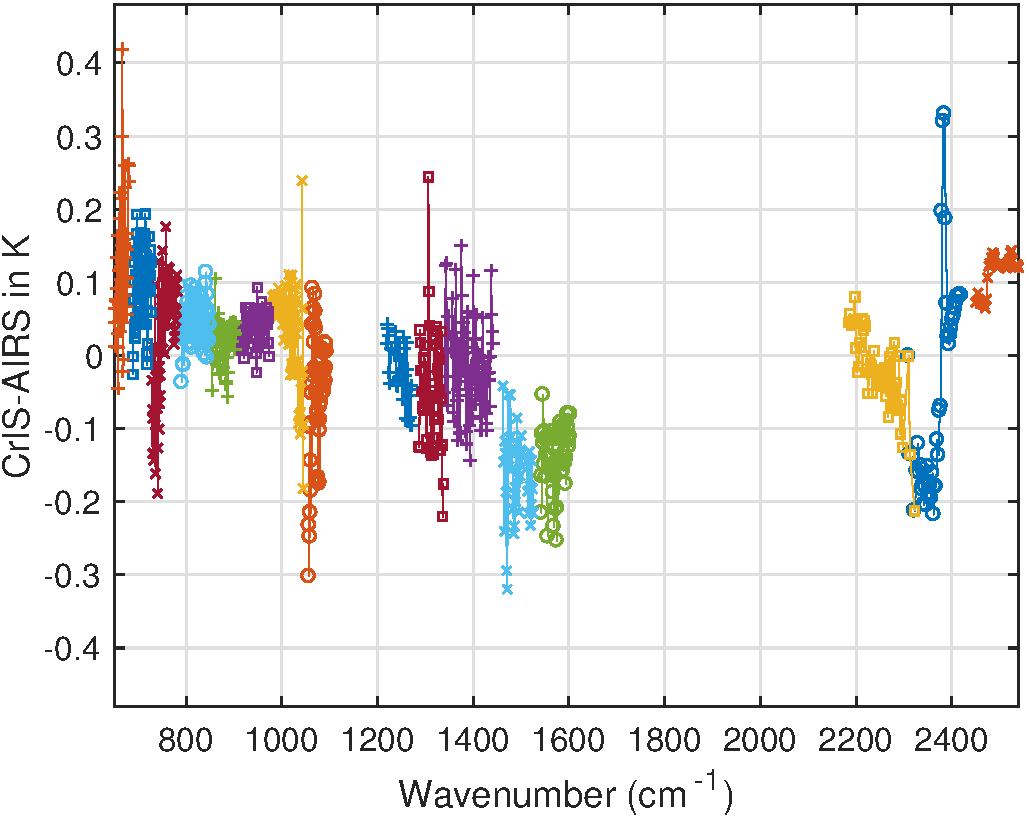
\includegraphics[width=\linewidth]{./Figs/Pdf/snpp_vs_airs_stats.pdf}
\end{center}
\end{block}
\end{column}
\end{columns}

\small
Sources for Differences
\vspace{-0.05in}
\begin{itemize}
\item Differential calibration AIRS modules
\item AIRS SRFs (widths and centroids)
\item Non-linearity: CrIS, AIRS?
\item etc.
\end{itemize}
\end{frame}

\begin{frame}[label={sec:org1908e31}]{SNPP vs NOAA20 CrIS (via AIRS Snos)}
\vspace{-0.1in}

\begin{center}
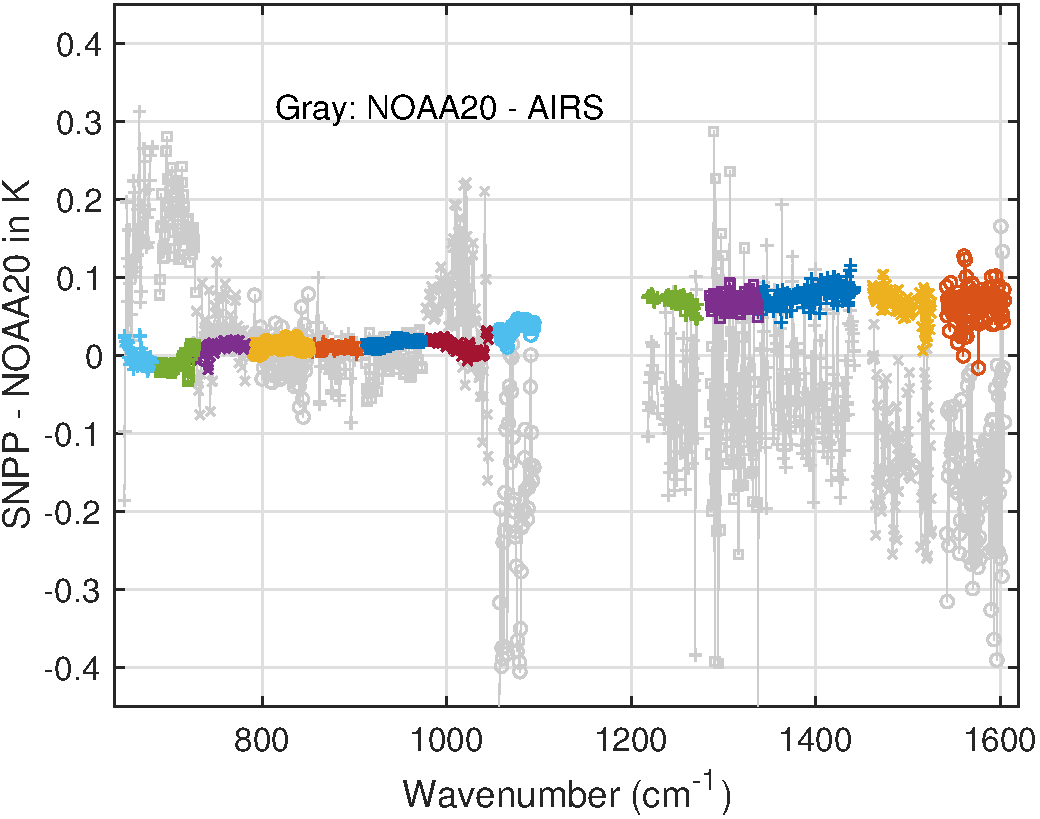
\includegraphics[width=0.65\linewidth]{./Figs/Pdf/sno_march2018_snpp_minus_noaa20_with_c2_airs_ingrey.pdf}
\end{center}

\vspace{-0.1in}

\small
\begin{itemize}
\item \emph{Preliminary}, NOAA20 CrIS non-linearity will be updated in July 2018
\item Connecting CrIS instruments together will be easier!
\item So far spatial, spectral, and sampling among CrIS instruments will be identical
\end{itemize}
\end{frame}

\begin{frame}[label={sec:orga29c98a}]{Time Series Tests}
(See talk by Chris Hepplewhite on Friday)
\begin{block}{Compared AIRS only to CHIRP Time Series}
\vspace{0.1in}
Start with a 1\% random subset of AIRS and CrIS observations:

\begin{itemize}
\item Series A: 10-year AIRS2CrIS time series trends
\item Series B: CHIRP (CrIS NSR SRF) 
\begin{itemize}
\item First 5-years is AIRS2CRIS
\item Second 5-years is CrIS
\end{itemize}
\item Correct AIRS2CrIS for radiometric offsets with CrIS
\item Intercompare 10-year trends between Series A and B
\end{itemize}

Results show climate level agreement between both. 

\vspace{0.1in}

Note: AIRS and CrIS do have sampling differences, very minimal with zonal averaging (which is what we did).
\end{block}
\end{frame}
\begin{frame}[label={sec:orge04a905}]{Pros of CHIRP}
\begin{itemize}
\item Only way I know to correct for inter-instrument radiometric offsets
\begin{itemize}
\item Certainly needed for AIRS vs CrIS+
\item Maybe needed for CrIS vs CrIS
\end{itemize}
\item Use of a single RTA for retrievals, using "same" channels
\item Use of a single Level 2 retrieval algorithm (noise issues, although these can be normalized)
\item Essential for providing a long-term Level-3 radiance data set of climate quality (next talk)
\item A simpler dataset for users in 20+ years
\item Lowers manpower efforts in a time of decreasing funding
\end{itemize}
\end{frame}

\begin{frame}[label={sec:orgf377716}]{Cons of CHIRP}
\begin{itemize}
\item Lowers spectral resolution of AIRS in the long-wave (after Hamming apodization)
\item Lowers spectral resolution of CrIS-FSR a little in the mid-wave, short-wave
\item \emph{If} you need similar noise figures, will need to add (a little) noise to either AIRS2CRIS or CrIS depending on the spectral region
\item The first two items may impact minor gas retrievals (\methane, HDO, CO) depending on the instrument
\item BUT, you can always "import" the native resolution radiances into your algorithm for the minor-gas part of the retrieval.  Adds complexity and a separate RTA.
\item Its new.
\end{itemize}
\end{frame}

\begin{frame}[shrink=20,label={sec:org31cb072}]{Future Work}
\begin{itemize}
\item AIRS L1c is a pre-requisite for AIRS2CrIS
\begin{itemize}
\item Ready except for frequency calibration (orbital + drift and Doppler corrections)
\item These should be ready in the next few months
\item UMBC can produce L1c with these corrections now
\item UMBC proposed L1c frequency set delivered to JPL
\end{itemize}
\item CHIRP Algorithm
\begin{itemize}
\item AIRS2CrIS is on github at \url{https://github.com/strow/airs\_deconv.git}
\item JPL SIPS is starting on integration and data formats
\item UMBC needs to formalize quality flags
\item Document performance 
\begin{itemize}
\item Algorithm paper accepted: Motteler et. a., IEEE Geophysical Transactions, 2018
\end{itemize}
\end{itemize}
\item CHIRP RTA
\begin{itemize}
\item UMBC has produced CrIS FSR=0.8/0.8/0.8 and NSR=0.8/0.4/0.2 OPD RTAs
\item However, they use different spectroscopy (FSR more up-to-date, HITRAN 2012)
\item We plan a new set of updates using HITRAN 2016 and new \cd-\water collision spectroscopy (see Sergio DeSouza-Machado's talk) in the next 6+ months?  Can also do CHIRP.
\item Similar plan for AIRS L1c RTA
\item Near term: could do proof-of-principle testing with CrIS NSR resolution for CHIRP
\end{itemize}
\end{itemize}
\end{frame}
\end{document}